\subsection{Ethernet controller driver}

\begin{frame}[fragile]{Ethernet driver endpoints}
	\begin{itemize}
		\item Ethernet controllers are represented by \kstruct{net_device}
		\item Entry points are the \kstruct{net_device_ops}
		\item Extra ethernet-specific callbacks implemented with \kstruct{ethtool_ops}
	\end{itemize}
	\begin{minted}{c}
dev->netdev_ops = &mvneta_netdev_ops;
dev->ethtool_ops = &mvneta_eth_tool_ops;
	\end{minted}
\end{frame}

\begin{frame}{Queues}
	\begin{columns}
		\column{0.3\textwidth}
		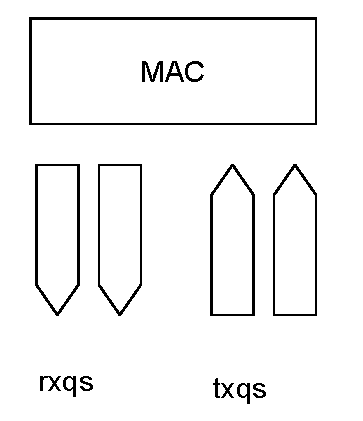
\includegraphics[width=\textwidth]{slides/networking-driver-netdev/queues.pdf}
		\column{0.7\textwidth}
	\begin{itemize}
		\item Most Ethernet controllers today have multiple \textbf{transmit} and \textbf{receive} queues
		\item \textbf{tx} queues hold \textbf{descriptors} for packets that are yet-to-be-sent
		\item The NIC will dequeue one packet at a time during transmission, from one of the tx queues
		\item The TX de-queueing behaviour can sometimes be controlled : Weighted Round-Robin, Per-queue priorities, etc.
		\item \textbf{rx} queues hold descriptors for packets received that weren't yet handled by the CPU
		\item the RX buffer size depends on the configured \textbf{MTU}
	\end{itemize}
	\end{columns}
\end{frame}

\begin{frame}[fragile]{RX filtering}
	\begin{itemize}
		\item The \textbf{receive filtering} is adjusted with :
	\begin{minted}{c}
void (*ndo_set_rx_mode)(struct net_device *dev);
	\end{minted}
	\item \code{dev->flags} contains the new filtering parameters :
		\begin{itemize}
			\item \code{IFF_PROMISC} : If set, the interface must go in \textbf{promiscuous mode}
			\begin{itemize}
				\item No hardware filtering of incoming frames must occur
				\item Used by tools like \code{tcpdump}, or \code{ip link set dev eth0 promisc on}
			\end{itemize}
			\item \code{IFF_ALLMULTI} : If set, all \textbf{multicast frames} must be accepted
		\end{itemize}
	\item The \textbf{unicast} and \textbf{multicast} address list must be updated :
		\begin{itemize}
			\item \code{dev->uc} contains all the Unicast addresses the interface must accept
			\item \code{dev->mc} contains all the Multicast addresses the interface must accept
		\end{itemize}
	\item The address list is maintained by the Networking stack, updated through \kfunc{dev_uc_add}, \kfunc{dev_uc_del}, \kfunc{dev_mc_add}, etc.
	\end{itemize}

\end{frame}

\begin{frame}[fragile]{Changing the MTU}
	\begin{itemize}
		\item \textbf{M}aximum \textbf{T}ransmit \textbf{U}nit, used by the upper layers for fragmentation
			\begin{itemize}
				\item Stored in \code{netdev->mtu}
			\end{itemize}
		\item User-modifiable with \code{ip link set dev eth0 mtu 1500}
			\begin{itemize}
				\item Triggers a call to the \code{.ndo_change_mtu} netdev ops
			\end{itemize}
		\item Changing the MTU may require the \textbf{re-allocation} of RX buffers in the queues
	\end{itemize}
	\begin{block}{\code{.ndo_change_mtu()} - option 1}
		{\fontsize{8}{9}\selectfont
		\begin{minted}{c}
if (netif_running(ndev
        return -EBUSY; /* Can't change the MTU while the interface is UP */

WRITE_ONCE(ndev->mtu, new_mtu);
		\end{minted}
		}
	\end{block}
	\begin{block}{\code{.ndo_change_mtu()} - option 2}
		{\fontsize{8}{9}\selectfont
		\begin{minted}{c}
WRITE_ONCE(ndev->mtu, new_mtu);

foo_stop_dev(dev); /* Stop sending and receiving, empty the queues*/
foo_realloc_queues(dev); /* Re-allocate buffers for the new MTU */
foo_start_dev(dev); /* Resume */
		\end{minted}
		}
	\end{block}
\end{frame}

\begin{frame}[fragile]{Channels}
	\begin{columns}
		\column{0.3\textwidth}
		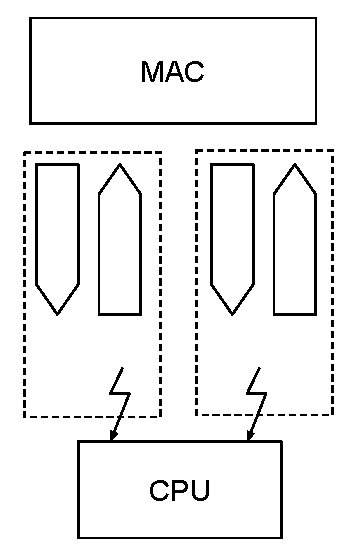
\includegraphics[width=\textwidth]{slides/networking-driver-netdev/channels.pdf}
		\column{0.7\textwidth}
	\begin{itemize}
		\item \code{tx} and \code{rx} queues will notify queueing and dequeueing through \code{interrupts}
		\item Multiple queues may share the same interrupt line
		\item A \textbf{channel} represents an interrupt line and its associated queues
		\item Channels can be added or removed, depending on hardware support
	\end{itemize}
		\begin{minted}{c}
void (*get_channels)(struct net_device *, struct ethtool_channels *);
int (*set_channels)(struct net_device *, struct ethtool_channels *);
		\end{minted}
	\end{columns}
\end{frame}

\begin{frame}{Receiving data}
	\begin{itemize}
		\item The receive path for a Ethernet Controller Driver must use the \textbf{NAPI} API
		\item The entry-point is an \textbf{interrupt handler} that will be called upon frame reception
		\item There may be multiple interrupts for RX (per-queue, per-cpu...)
		\item NAPI mandates a short \textbf{top half} that acknowledges the interrupt and \textbf{masks it}
		\item The handler then calls \kfunc{napi_schedule}.
		\item Most of the processing occurs in \textbf{softirq} context, on the \textbf{same CPU} that handled the interrupt
	\end{itemize}
\end{frame}

\begin{frame}{NAPI principle}
	\begin{itemize}
		\item NAPI does \textbf{not} stand for \textbf{N}ew \textbf{API}
			\begin{itemize}
				\item it was new in Linux v2.4, today NAPI means NAPI
			\end{itemize}
		\item Designed to avoid interrupt interference, as traffic often occurs in bursts
		\item The \textbf{first packet} of a burst is handled through interrupt
		\item The interrupt stays disabled, each subsequent packet is pulled using \textbf{polling}
		\item The polling stops when the \textbf{budget} is exhausted (by default, 50 packets)
		\item The driver must then re-enable the interrupts for further processing
		\item NAPI is not a batch processing mechanism, which is achievable through \textbf{interrupt coalescing}
	\end{itemize}
\end{frame}

\begin{frame}{NAPI Loop}
	\begin{itemize}
		\item Register the NAPI polling function (per-queue) : \code{netif_napi_add}
		\item Polling function runs in \textbf{softirq} context : \textbf{Cannot sleep}
	\end{itemize}
	\begin{enumerate}
		\item Hardware IRQ fires upon receiving a first packet
		\item IRQ handler disables interrupts for that queue, and calls \code{napi_schedule}
		\item The NAPI system calls the polling function \code{int (*poll)(struct napi_struct *napi, int budget}
		\item Each received frame counts as \textbf{1} budget item
			\begin{itemize}
				\item If the budget is exhausted but there are still packets to process, return \code{budget}
				\item The polling function may be called with a budget of \code{0}, for TX processing only
			\end{itemize}
		\item If the budget isn't exhausted but all packets are processed, call \code{napi_complete_done()} and unmask interrupts
	\end{enumerate}
\end{frame}

\begin{frame}[fragile]{NAPI instances}
	\begin{itemize}
		\item NAPI poll handlers are registered with \kfunc{netif_napi_add}
		\item Multiple NAPI \textbf{instances} can be registered
			\begin{itemize}
				\item Usually one per \textbf{channel} or per \textbf{CPU}
			\end{itemize}
	\end{itemize}
	\begin{block}{napi .poll()}
		\begin{minted}{c}
static int foo_poll(struct napi_struct *napi, int budget)
{
    while(rx_done < budget) {
        buff = foo_queue_get_next_desc();
        foo_do_xdp(buff);
        skb = foo_build_skb(buff);
        napi_gro_receive(skb);
        rx_done++;
    }
}
		\end{minted}
	\end{block}
\end{frame}

\begin{frame}{Interrupt Coalescing}
	\begin{itemize}
		\item \textbf{Hardware feature} where the MAC waits for multiple packets to be received before triggering the interrupt
		\item Users configure a number of pending packets and a timeout for RX interrupt generation
		\item Must be fine-tuned depending on the use-case :
			\begin{itemize}
				\item High threshold allows batching the interrupts, suitable for high-throughput workloads
				\item Low threshold allows triggering interrupts as soon as data is received, for low-latency workloads
			\end{itemize}
		\item \code{ethtool -C eth0 adaptive-rx on adaptive-tx on tx-usecs-irq 50}
		\item Software IRQ coalescing also exists, using NAPI and a polling-rearm timer
	\end{itemize}
\end{frame}

\begin{frame}{Transmit path}
	\begin{itemize}
		\item Packets are sent from a network controller through the \code{.ndo_start_xmit} callback
			\begin{itemize}
				\item \code{netdev_tx_t .ndo_start_xmit(struct sk_buff *skb, struct net_device *dev)}
				\item it is the only mandatory \code{net_device_ops} member !
			\end{itemize}
		\item The \code{.ndo_start_xmit()} callback enqueues and sends the \code{skb}
		\item If the skb is fragmented, all fragments must be sent
		\item In case of an error, the \code{skb} is dropped, but we still return \code{NETDEV_TX_OK}
		\item The \code{dev->stats} and driver-specific counters must be updated
	\end{itemize}
\end{frame}

\begin{frame}{NAPI TX}
	\begin{itemize}
		\item TX \textbf{completions} are handled in the NAPI loop
		\item The driver acknowledges that packets were correctly sent
		\item During a NAPI poll, drivers are free to acknowledge as many TX packets as they want
		\item \code{budget} does not apply to TX packets
			\begin{itemize}
				\item The NAPI poll function can acknowledge as many TX packets as it wants
			\end{itemize}
	\end{itemize}
\end{frame}

\begin{frame}{Buffer management}
	\begin{itemize}
		\item Hardware queues contain pre-populated \textbf{dma descriptors}
		\item On the receive side, when receiving packets the queues must be \textbf{refilled}
		\item Usually done at the end of the NAPI loop
		\item This is driver specific, but the buffers can be kept in \textbf{pools}
	\end{itemize}
\end{frame}

\begin{frame}{Page pool}
	\begin{itemize}
		\item Page pools allows fast page allocation without locking
		\item One \code{struct page_pool} must be allocated per-queue
		\item Getting a page from \code{page_pool} happens without locking
		\item This is only used on the \textbf{receive} side
		\item Using \code{page_pool} is strongly recommended to support \textbf{XDP}
		\item See the \href{https://docs.kernel.org/networking/page_pool.html}{page pool documentation}
	\end{itemize}
\end{frame}

\begin{frame}{Timestamping}
	\begin{itemize}
		\item Packet timestamping can be done in RX and TX
		\item Hardware timestamping is configured in the \code{.ndo_ioctl()}
			\begin{itemize}
				\item Being replaced in favor of \code{.ndo_timestamping()}
			\end{itemize}
		\item Timestamp is stored in the \code{skb_shared_info}
		\item On TX timestamping, the \code{skb} is cloned, timestamp is attached to the clone
			\begin{itemize}
				\item The clone is sent back to the \textbf{socket error queue}
			\end{itemize}
	\end{itemize}
\end{frame}

\begin{frame}{Netdev features}
	\begin{itemize}
		\item \code{features} represents hardware offload capabilities
			\begin{itemize}
				\item Checksumming, Scatter-gather, segmentation, filtering (mac / vlan)
				\item see \code{ethtool -k <iface>}
				\item attributes of \code{struct net_device}
			\end{itemize}
		\item Drivers set \code{netdev.hw_features} at init, and can also set \code{netdev.features}
			\begin{itemize}
				\item \code{features} : The current active features
				\item \code{hw_features} : Features that can be changed (\textit{hw != hardware})
			\end{itemize}
		\item Users but also the core might want to change the enabled features
			\begin{itemize}
				\item Child devices might require some features to be disabled
			\end{itemize}
		\item \code{.ndo_fix_features()} filters incompatible feature sets for the driver
		\item \code{.ndo_set_features()} applies the new feature set
		\item \url{https://docs.kernel.org/networking/netdev-features.html}
	\end{itemize}
\end{frame}

\begin{frame}{Offloading}
	\begin{itemize}
		\item Most modern controllers can perform themselves some operations on packets
		\item \textbf{checksumming} offload makes so the CPU doesn't have to check or compute checksums
		\item \textbf{filtering} offloads makes so that the MAC drops unknown MAC addresses and VLANs
		\item \textbf{classification}-capable controllers may implement more powerful features :
			\begin{itemize}
				\item \textbf{header hashing} computes a hash of a specific set of fields in the header. Useful for RSS.
				\item \textbf{flow steering} allows specific actions (enqueueing, drop, redirection) to be done based on specific header values
			\end{itemize}
		\item \textbf{crypto} offload for some tunneling technologies such as MACSec
		\item Offloading can however make debugging harder, as decisions are taken before packets reach the CPU
			\begin{itemize}
				\item Most controllers will expose counters, accessible over \code{ethtool -S <iface>}
			\end{itemize}
	\end{itemize}
\end{frame}

\begin{frame}{Checksumming}
	\begin{itemize}
		\item Some protocols include a checksum of the header or payload in the frame
			\begin{itemize}
				\item Ethernet has the \textbf{FCS} that checksums the whole frame
				\item IPv4 header includes a Header Checksum for the IPv4 header itself
				\item TCP and UDP checksums the header and the payload
			\end{itemize}
		\item Checksum computation and verification need to be done for every frame
		\item Some devices can compute and verify checksums at the hardware level
		\item TX checksumming involves computing the checksum of a section of the packet, and editing the checksum inline
		\item \textbf{caution :} Outgoing traffic will be shown with wrong checksums in captures
	\end{itemize}
\end{frame}

\begin{frame}{RSS}
	\center{\textbf{R}eceive \textbf{S}ide \textbf{S}teering}
	\begin{itemize}
		\item Hardware feature on the \textbf{receive} side to spread traffic handling across queues and cores
		\item Requires per-queue or per-cpu interrupt support in the Ethernet controller
		\item Incoming packets can't be arbitrarily steered to any CPU or queue
			\begin{itemize}
				\item Risk of out-of-order delivery, and bad caching behaviour
			\end{itemize}
		\item The hardware parses the packet header and computes a hash of some of its fields
			\begin{itemize}
				\item Usually CRC32 or Toeplitz
			\end{itemize}
		\item The Hash is then used as a lookup index in a RSS table to get the RX queue
		\item \code{.get_rxfh} and \code{.set_rxfh}
	\end{itemize}
\end{frame}

\begin{frame}{XPS}
	\begin{itemize}
		\item Associate TX queues with CPU cores
		\item Frames enqueued from a given core always go in the same queue
		\item Avoids contention on enqueueing
			\begin{itemize}
				\item Each CPU can enqueue without cross-CPU locking
			\end{itemize}
		\item Optimizes the completion handling
		\item \code{netif_set_xps_queue(dev, cpumask_of(queue), queue);}
	\end{itemize}
\end{frame}

\begin{frame}{Flow steering}
	\begin{itemize}
		\item Advanced controllers have the ability to \textbf{parse} packet headers
		\item This is complex, as the header fields are not at fixed offsets (presence of VLAN tags, encapsulation, etc.)
		\item This is usually achieved with internal \textbf{TCAM-based lookup engines}
		\item Traffic is classified based on specific fields : src/dst MAC, src/dst IP, src/dst Port, VLAN, etc.
		\item Classified traffic are assigned actions :
			\begin{itemize}
				\item Drop (DoS mitigation)
				\item Redirection
				\item Enqueueing
				\item Policing (rate limiting)
			\end{itemize}
	\end{itemize}
\end{frame}

\begin{frame}[fragile]{TC and ethtool steering}
	\begin{itemize}
		\item Flow steering can be offloaded via \code{ethtool} :
			\begin{minted}{bash}
ethtool -K eth0 ntuple on
ethtool -N eth0 flow-type tcp4 vlan 0xa000 m 0x1fff action 3 loc 1
			\end{minted}
		\item Steers Vlan-tagged TCP over IPv4 with priority 6 (\code{0xa000 & 0x1fff}) in queue 3
		\item Implemented in the \code{.set_rxnfc} ethtool op, \textit{e.g.} \kfunc{mvpp2_ethtool_set_rxnfc}
		\item Can also be done with \textbf{tc flower}
			\begin{itemize}
				\item Through \code{.ndo_setup_tc}
			\end{itemize}
		\item Both APIs use the same representation : \kstruct{flow_rule}
	\end{itemize}
\end{frame}

\begin{frame}{Multi-queue and priorisation}
	\begin{itemize}
		\item Some Ethernet Controllers have multiple \code{tx} and\code{rx} queues
		\item On the \textbf{transmit} side, allow shaping and priorizing traffic
		\item On the \textbf{receive} side, allow load-balancing and per-queue actions
		\item flows can be assigned to dedicated \textbf{rx queues}
		\item These queues can in turn be pinned to CPUs, apps, VMs, or be rate-limited.
		\item Most of this is controlled through \textbf{tc} in \code{.ndo_setup_tc}
		\item Example in \kfunc{mvneta_setup_mqprio}
	\end{itemize}
\end{frame}

\begin{frame}{Other \kstruct{ethtool_ops}}
	\begin{itemize}
		\item \code{.get_ringparam} and \code{.set_ringparam}
			\begin{itemize}
				\item Adjust the size of queues
			\end{itemize}
		\item \code{.get_strings} and \code{get_ethtool_stats}
			\begin{itemize}
				\item Returns hardware stats
			\end{itemize}
		\item \code{.get_link_ksettings} and \code{set_link_ksettings}
			\begin{itemize}
				\item Get the link speed and duplex
				\item Usually the driver queries the PHY driver to get this information
			\end{itemize}
		\item \code{.get_wol} and \code{.set_wol}
			\begin{itemize}
				\item Configure Wake-on-Lan
			\end{itemize}
	\end{itemize}
\end{frame}

% Netdev ops
% Receive path + NAPI
% Transmit path
% Netdev features
% Buffer management + page pool
% Queue management
% Timestamping
% Ethtool ops and link reporting
% Offloading (TC, ethtool, features)

